\section{Durchschnittliche Verschiebung im nationalen Vergleich}
In den folgenden Abbildungen sind die deutschen Landkreise und Regierungsbezirke wie in \autoref{sec:BeschreibungKorrelationsanalyse} beschrieben dem Durchschnitt der Werte ihrer Zeile in der beschriebenen Matrix eingefärbt.
\subsection{Verteilung der durchschnittlichen Verschiebung unter den Landkreisen}\label{sec:Durchführung:Verteilung der durchschnittlichen Verschiebung unter den Landkreise}
In \autoref{fig:average_shift_counties.png} sind die Landkreise entsprechend des Mittels ihrer Zeilen in der rechten unteren Matrix aus \autoref{fig:matrizes_pop_density_counties} beziehungsweise \autoref{fig:matrizes_north_to_south_counties} eingefärbt. Die Zeilen der Matrizen enthalten die Verschiebungen $\tau_0$, die unter allen Verschiebungen $\tau\in [-30,30]$ den höchsten Wert $c(\tau)$ bei der Korrelationsanalyse des Landkreises der Zeile mit dem Landkreis der Spalte erzeugen.

\begin{figure}[H]
    \centering
    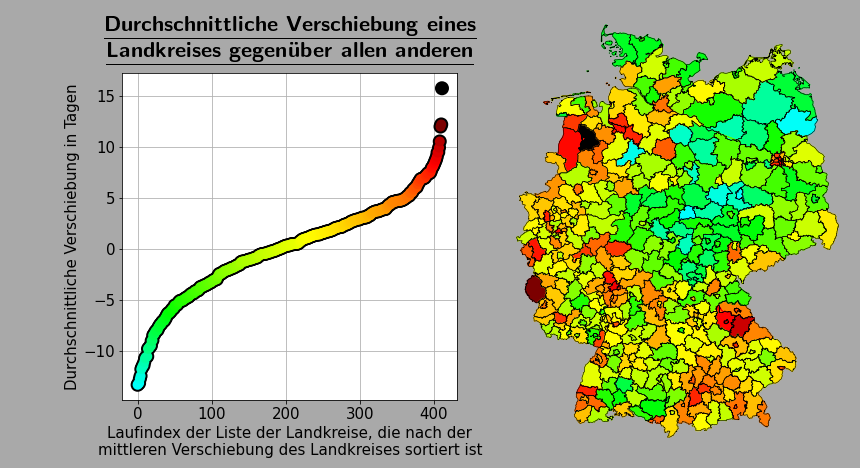
\includegraphics[width = \textwidth]{figures/Ergebnisse/average_shift_counties.png}
    \caption{Mittel der maximalen Verschiebungen $\overline{\tau}$ eines Landkreises gegenüber allen anderen. Dieser wird nach \autoref{eq:Mittelwert} berechnet. Links ist die Verteilung der Mittel der maximalen Verschiebungen $\overline{\tau}$ und die Farbgebung gezeigt. Rechts ist die räumliche Verteilung dargestellt.}
    \label{fig:average_shift_counties.png}
\end{figure}
\newpage
Auch in \autoref{fig:positive_or_negative_shift_counties} sind die Landkreise entsprechend dem Mittel ihrer Zeilen in einer Matrix eingefärbt. Hierzu wurden jedoch die Werte aus der rechten oberen Matrix in \autoref{fig:matrizes_pop_density_counties} beziehungsweise \autoref{fig:matrizes_north_to_south_counties} verwendet. Die Zeilen der Matrizen enthalten die Tendenzen der Verschiebung $\hat{\tau}$ die aus den Korrelationswerten $c(\tau)$ der Verschiebungen $\tau\in [-30,30]$ berechnet werden.

Die Karte ähnelt der Deutschlandkarte in \autoref{fig:average_shift_counties.png} sehr:
Auch hier ist ein Ost-West-Verlauf festzustellen, wie bereits in \autoref{sec:Durchführung:Korrelationsmatrizen sortiert nach der Bevölkerungsdichte} ausgeführt. Einzig Bayern und Berlin stellen Ausnahmen dar, da sie überwiegend positive Werte enthalten.

\begin{figure}[H]
    \centering
    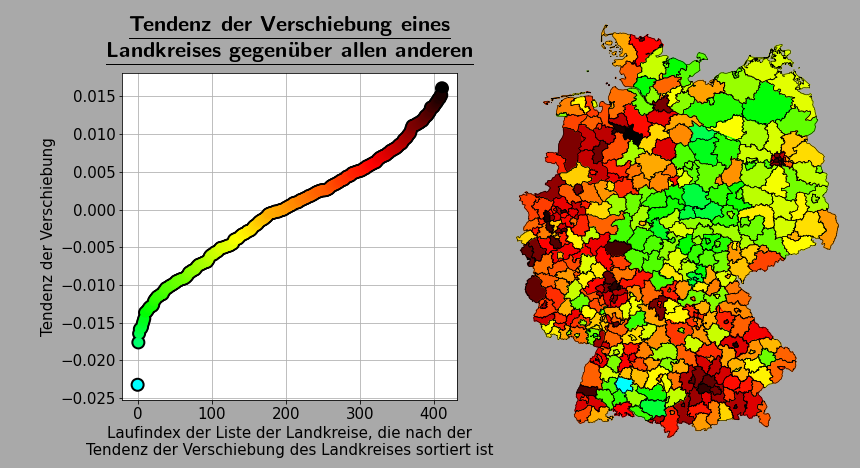
\includegraphics[width = \textwidth]{figures/Ergebnisse/positive_or_negative_shift_counties.png}
    \caption{
    Mittel der Tendenzen der Verschiebung $\overline{\hat{\tau}}$ eines Landkreises gegenüber allen anderen. Dieser wird nach \autoref{eq:Tendenz der Verschiebung} und \autoref{eq:Mittelwert} berechnet. Links ist die Verteilung der Mittel der Tendenzen der Verschiebung $\overline{\hat{\tau}}$ und die Farbgebung gezeigt. Rechts ist die räumliche Verteilung dargestellt.}
    \label{fig:positive_or_negative_shift_counties}
\end{figure}


\newpage
\subsection{Verteilung der durchschnittlichen Verschiebung unter den Regierungsbezirken}\label{sec:durchführung:Verteilung der durchschnittlichen Verschiebung unter den Regierungsbezirken}



In \autoref{fig:average_shift_districts.png} sind die Regierungsbezirke entsprechend der Durchschnitte ihrer Zeilen in der rechten unteren Matrix aus \autoref{fig:matrizes_pop_density_districts} beziehungsweise \autoref{fig:matrizes_north_to_south_districts} eingefärbt. Die Zeilen der Matrizen enthalten die Verschiebungen $\tau_0$, die unter allen Verschiebungen $\tau\in [-30,30]$ den höchsten Wert $c(\tau)$ bei der Korrelationsanalyse des Regierungsbezirks der Zeile mit dem Regierungsbezirk der Spalte erzeugen.

Der bereits mehrfach angesprochene Ost-West-Verlauf ist auch hier festzustellen. Die in \autoref{sec:Durchführung:Verteilung der durchschnittlichen Verschiebung unter den Landkreise} angesprochenen Ausnahmen Bayern und Berlin sind auch hier klar zu erkennen.

\begin{figure}[H]
    \centering
    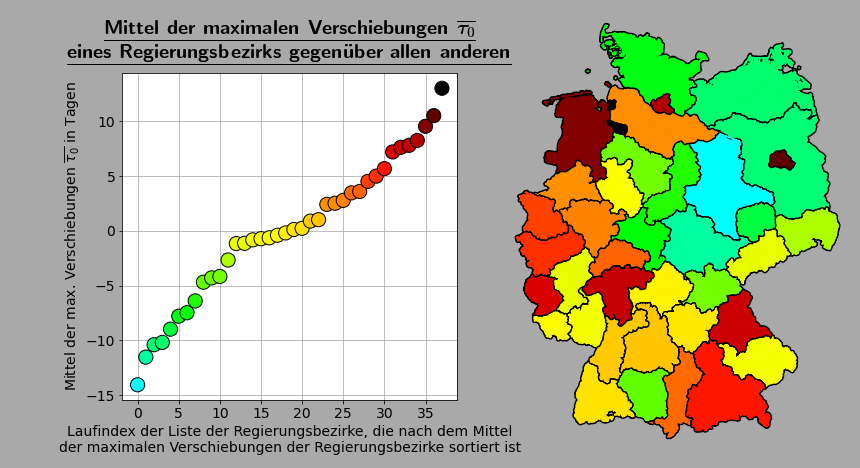
\includegraphics[width = \textwidth]{figures/Ergebnisse/average_shift_districts.png}
    \caption{Mittel der maximalen Verschiebungen $\overline{\tau}$ eines Regierungsbezirks gegenüber allen anderen. Dieser wird nach \autoref{eq:Mittelwert} berechnet. Links ist die Verteilung der Mittel der maximalen Verschiebungen $\overline{\tau}$ und die Farbgebung gezeigt. Rechts ist die räumliche Verteilung dargestellt.}
    \label{fig:average_shift_districts.png}
\end{figure}
\newpage
Auch in \autoref{fig:positive_or_negative_shift_districts} sind die Regierungsbezirke entsprechend dem Mittel ihrer Zeilen in einer Matrix eingefärbt. Hierzu wurde jedoch die Werte aus der rechten oberen Matrix in \autoref{fig:matrizes_pop_density_districts} beziehungsweise \autoref{fig:matrizes_north_to_south_districts} verwendet. Die Zeilen der Matrizen enthalten die Tendenzen der Verschiebung $\hat{\tau}$ die aus den Korrelationswerten $c(\tau)$ der Verschiebungen $\tau\in [-30,30]$ berechnet werden.

Diese Karte ähnelt der Deutschlandkarte in \autoref{sec:durchführung:Verteilung der durchschnittlichen Verschiebung unter den Regierungsbezirken} ziemlich.

\begin{figure}[H]
    \centering
    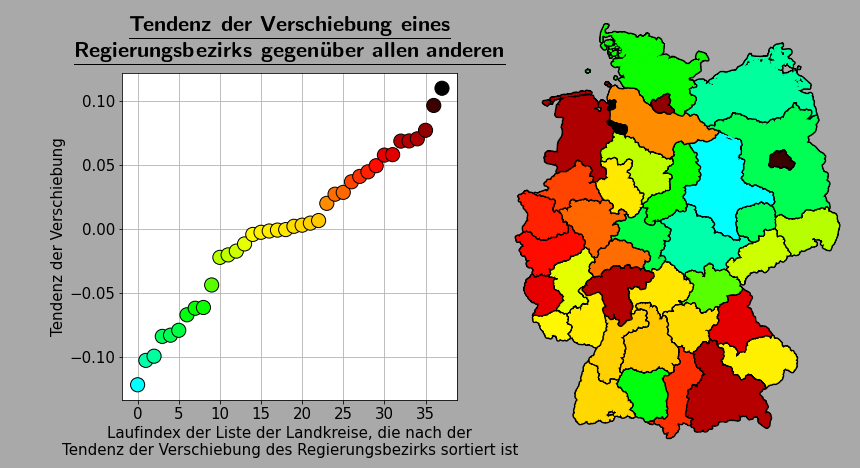
\includegraphics[width = \textwidth]{figures/Ergebnisse/positive_or_negative_shift_districts.png}
    \caption{
    Mittel der Tendenzen der Verschiebung $\overline{\hat{\tau}}$ eines Regierungsbezirks gegenüber allen anderen. Dieser wird nach \autoref{eq:Tendenz der Verschiebung} und \autoref{eq:Mittelwert} berechnet. Links ist die Verteilung der Mittel der Tendenzen der Verschiebung $\overline{\hat{\tau}}$ und die Farbgebung gezeigt. Rechts ist die räumliche Verteilung dargestellt.}
    \label{fig:positive_or_negative_shift_districts}
\end{figure}

